%---Introduction to the MDA and how it basically works
\section{Model Driven Engineering (MDE)}
\label{ModelDrivenEngineering}
Model Driven Engineering (MDE) is a development methodology which focuses on creating models rather than algorithmic concepts that are usually addressed in the classical programming approaches.
This discipline attempts an abstraction of the benefits and the features provided by the Software Engineering \cite{Marrone}, usually creating a domain specific framework for implementing new systems, based on well known and tested concepts, obtained through a careful and detailed analysis of the domain and its actors.\\
%
MDE essentially shifts the focus from the program code to models, making them the gravitational center of every MDE process \cite{Lukman08}. The model represents the system and the language which describes the model must be characterized by a well defined syntax and semantic. This way, if the model strictly complies with the languages' rules, it is possible to create automatized routines that carry out activities such as debugging, validation, simulation or transformation \cite{Papa11}. 
The language to describe the model is itself complying with a meta-model which, recursively, complies with a meta-meta-model. In fact, a typical MDE approach consists of the usage of a pile of models having at the top the system model. \\
%
Eventually, the two main principles of MDE are:
\begin{itemize}
 \item creation of models: using meta-modelling techniques
 \item automatized manipulation of models: using transformations to transform an input model (conforming to a source meta-model) to an output model (conforming to a destination meta-model)
\end{itemize}

\subsection{Model Driven Architecture (MDA)}
\label{MDA}
Actually, the MDE concepts are generic and can be applied to many engineering disciplines where models are used. To narrow our attention down to software development, we should consider the Model Driven Architecture (MDA), which is a standard from the Object Management Group (OMG) that specifies in details the particular modeling languages (e.g. UML) and the related automations to map an input model into an output one.
A very common MDA pattern consists of the definition of three models \cite{Marrone} representing the input application, the platform information and the output application:

\begin{itemize}
 \item Platform Independent Model (PIM): it is a model of the application, completely independent from the platform on which it might be implemented
 \item Platform Description Model (PDM): it describes the architecture on which the output application should be deployed
 \item Platform Specific Model (PSM)$=f($PIM,PDM$)$: it is the result of an automatic transformation of the PIM using the PDM specific platform directives  
\end{itemize}

The output models, result of the MDA transformations, are so called: "correct-by-construction" models, in opposition to some traditional transformations that are of a "construct-by-correction" type \cite{Marrone}.   


\subsection{MDA: the manipulation of models}
\label{MDAModelManipulation}
Among the automated routines that MDA can perform on models, we focus on the model Transformations, that, starting from an input model, create an output model conforming to a destination meta-model. 

\paragraph{Transformations of models}
As described in \cite{Papa11}, a transformation is formed by a set of rules, or \textbf{transformation rules}, that describe how an element expressed in the source language should be transformed in one or more elements of the destination language.
Of course, both the source and destination model must comply with their respective meta-models.
%FIXME add a picture like the one in http://www.ebpml.org/blog/130.htm
The possible transformation rules that can be applied to a model depend on the approaches being used \footnote{Some approaches come from the scientific literature, some in response to the OMG's requests for proposals and others from open-source or commercial vendors.}. Czarnecki and Helsen \cite{Czarnecki03classificationof} classify and describe the set of rules common to all the approaches.
They individuate the main rules that compose a model transformation; these rules span from defining how to transform and with which scope to scheduling and organizing the transformation.

\subsubsection{Model-to-Model and Model-to-Text transformations}
\label{m2m&m2t}
Depending on the kind of source model\footnote{other techniques, not model-based (XML document to XML document, Text-to-Binaries, etc.), can also be abstracted under the generic type of model transformations \cite{M2TandM2M}} , there are two kinds of transformations \cite{Papa11}: \textbf{Model-to-Model} and \textbf{Model-to-Text} (or Model-to-Code, when the output text is a programming language syntax.). Both the transformations can be implemented in two ways \cite{M2TandM2M}:
\begin{itemize}
 \item Using a model Domain-Specific Modeling Language (DSML)
 \item Using a General Purpose Language (GPL), e.g. Java, C\#
\end{itemize}
The difference is that a domain specific modeling language focus on a particular application domain thus it can represent concepts that are not possible to describe with a general purpose language.
For both these transformations, the OMG created standard specifications: the QVT (Query/View/Transformation) specification for the model-to-model and the MOFM2T (MOF Model to Text Transformation language) specification for the model-to-text. These specifications belong to the OMG's Model-Driven Architecture

\paragraph{Model-to-Text approaches}
If we have a deeper look in the Model-to-Text transformations, we notice that Czarnecki and Helsen \cite{Czarnecki03classificationof} subdivide this category in two: Visitor-based and Template-based transformations.
\subparagraph{Visitor-Based model-to-text transformation}
It is a simple method where a visitor mechanism can traverse the model's internal architecture and directly write text as output, deciding what transformation to apply depending on the construct encountered. 
\subparagraph{Template-Based model-to-text transformation}
This approach represents the most used M2T technique. It contains code templates in which some portions of code are left blank, waiting to be filled with information coming from the input model. 
The templates comply to the output meta-model, and resembles the code to be generated. 
In the template-based transformations, there also are multiple mechanisms to gather the information (from the source model) to insert in the templates. A common way is to describe the source model with a non-ambiguous language and later access it through an API provided by the creators of the modeling language. Declarative queries can also be used, as it happens with the Object Constraint Language (OCL) or XML PAth Language (XPath). 
More advanced techniques implement a hybrid solution, using a mix templates and more complex queries to get data from different parts of the source model.  
%{I templates in Acceleo sono scritti nel linguaggio di destinazione (Java nel nostro caso) + snippets di codice Acceleo. In generale, i templates sono (sempre?) scritti nel linguaggio di destinazione? }

\subsubsection{The role of a meta-model in a transformation: Meta-modeling}
\label{Meta-modeling}
If a model is a schematic representation of reality, a meta-model can be thought of as a model of a model \cite{AcceleoUserGuide}.
Metamodelling is a vast domain and has been formalized by OMG with the creation of the Meta-Modeling Facilities (MOF).
MOF is itself a model, represented as a tree. It is considered a meta-meta-model as it can be used to describe many other meta-models. This is possible thanks to the fact that its components are basic, and form the atomic pieces used to create other models. 
For example, if a map represents a model of a region, existing in the real world, its meta-model would contain the basic elements to represent such a map, namely, a legend. This meta-model would contain elements such as roads, highways, rivers, cities, villages etc. In this context, a meta-meta-model would go further deep in the description, containing the structure of the atomic elements to represent the elements of the meta-model (the legend); for example, of a river, it would present a model containing name, depth, length, etc.  
Basically, a model is an instance of a meta-model \cite{UnderstandMetamodelling}. 

\paragraph{An example of a real meta-model}
\label{metamodelExample}
In a transformation a meta-model defines the structure of the input language, or better, what the elements we can expect to work with are. As a practical example of a meta-model, we could think of a UML-like model, where there are defined the main classes of elements, the attributes, the inheritances, the relations of inclusion etc. Meta-models are usually provided by the proprietaries of a technology or, as in the case of the Eclipse Modeling Framework (read Section \ref{EMF} for more details), they are all written using a standard meta-meta-model called Ecore (which is a dialect of UML \cite{EcoreAPI}). In fact, there are available ecore meta-model for almost any programming language. What is more, if one invents his own language to describe a custom process or his company positions' tree, with a well defined set of elements and hierarchy, he can easily create his own ecore meta-model \cite{EcoreExample}.

To give a real example of meta-model, Figure \ref{BPELEcoreExample} represents a very small (yet not complete) part of the entire BPEL meta-model. It shows some of the elements of the BPEL language and how they relate to each other. The \textit{Assign} element is composed by \textit{Copy} elements, which always contains a \textit{From} and a \textit{To}. The power of a meta-model relies in the fact that it makes it possible to access, directly, any of the elements, sub-elements and attributes composing an input file. To conclude the example, if our purpose would be to transform a BPEL input file to a Java file, we could easily imagine how to translate a BPEL \textit{Assign} element (which assigns a value to a variable) in a Java "\textit{=}" operation: the value of the \textit{To} element should be equal to the value of the \textit{From}. 

\begin{figure}
  \begin{center}
    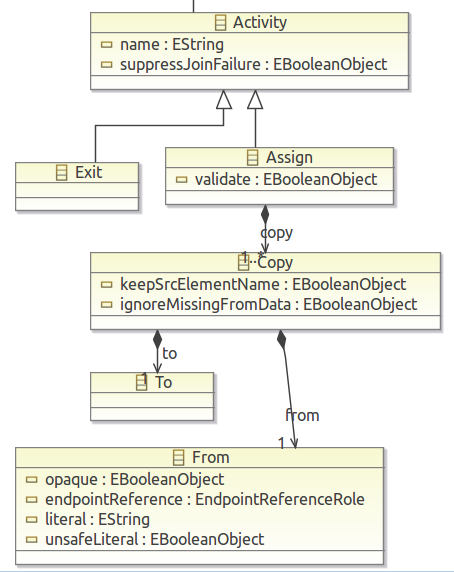
\includegraphics[scale=0.5]{pictures/BPELMetaModelExample.png}
    \caption{A small part of the BPEL.ecore meta-model, representing the inheritance relations of an Assign Activity, its composing elements: Copy and the Copy's composing elements: From and To}
    \label{BPELEcoreExample}
  \end{center}
\end{figure}

\subsubsection{The Eclipse Modeling Framework (EMF)}
\label{EMF}
Among the languages and frameworks that provide tools and techniques to manage models, the Eclipse Modeling Framework is surely one of the most widespread. 
EMF is a modeling framework and code generator created by the Eclipse Foundation. It provides facilities to define models (written in any modeling language such as XML, UML, etc.), transform these models in other type of models and, last but not least, generate code from the models. The final aim of EMF would be that "modeling and programming can be considered the same thing" \cite{Steinberg2009EMF}. The meta-model used by EMF to describe any model is called Ecore and has itself, recursively, a meta-meta-model defining its parts. 

One of the most important characteristic of EMF is that it fully supports XML Metadata Interchange (XMI) serialization. XMI can be thought as a way to save models in XML, yet it is much more powerful than that: it shows how to save any MOF-based meta-model in XML \cite{XMIandMOF}. The of XMI serialization's success is that it takes advantage of the dominance in the software design world of UML (which has a MOF meta-model) and the widespread usage of XML. It practically permits to export models and make them usable on several modeling frameworks and languages; it also act like a bridge between transformations from an input model to a different output model.


%---- XMI is the standard from OMG to transform, interchange, and express any model realized with the MOF.   

% Acceleo M2T
\subsection{Acceleo FIXME: to move and complete}
\label{acceleo}

General Info about meta-modelling   :Pag7 \cite{AcceleoUserGuide}

- MEtamodelling is a vast domain
--- MetaModelling has been formalizaed by OMG, known as MOF Meta-Modeling Facilities
----- MOF is itself a model, represented as a tree. It is considered a meta-meta-model as it can be used to describe many other meta-models. This is possible thanks to the fact that its components are basic, and form the atomic pieces used to create other models. 
For example, if a map represents a model of a region, existing in the real world, its meta-model would contain the basic elements to represent such a map, namely, a legend. This meta-model would contain elements such as roads, highways, rivers, cities, villages etc. In this context, a meta-meta-model would go further deep in the description, containing the structure of the atomic elements to represent the elements of the meta-model (the legend). For example, of a river, it would present a modelization of it, containing name, depth, length and more.  

Basically, a model is an instance of a meta-model \cite{UnderstandMetamodelling}. 


---- XMI is the standard from OMG to transform, interchange, and express any model realized with the MOF.   
   

% The best known MDE initiative is the Object Management Group (OMG) initiative Model-Driven Architecture (MDA), which is a registered trademark of OMG \cite{MDE}.
% 
% It is generic and groups all of the more specific techniques to develop something using models. This something can be software, ...etc.
% The objective: define methodologies and techniques to support software development through models manipulation.


% \subsection{The Model Driven Architecture (MDA)}
% \label{MDA}
% 
% \subsubsection{Model Driven Engineering}
% \label{MDE}
% \subsubsection{Model to Text transformation (M2T)}
% \label{M2T}
% \subsubsection{Acceleo}
% \label{Accelelo}

%- What it is \nl
%- Why we use it, why is good (because it is generic, Architecture independent, Reuse)  \nl
%- How we use it: From BPEL processes to Java RMI processes \nl

 
